\newcommand{\FigBentSolenoidRelativeDrift}{
\begin{figure}[t]
\centering
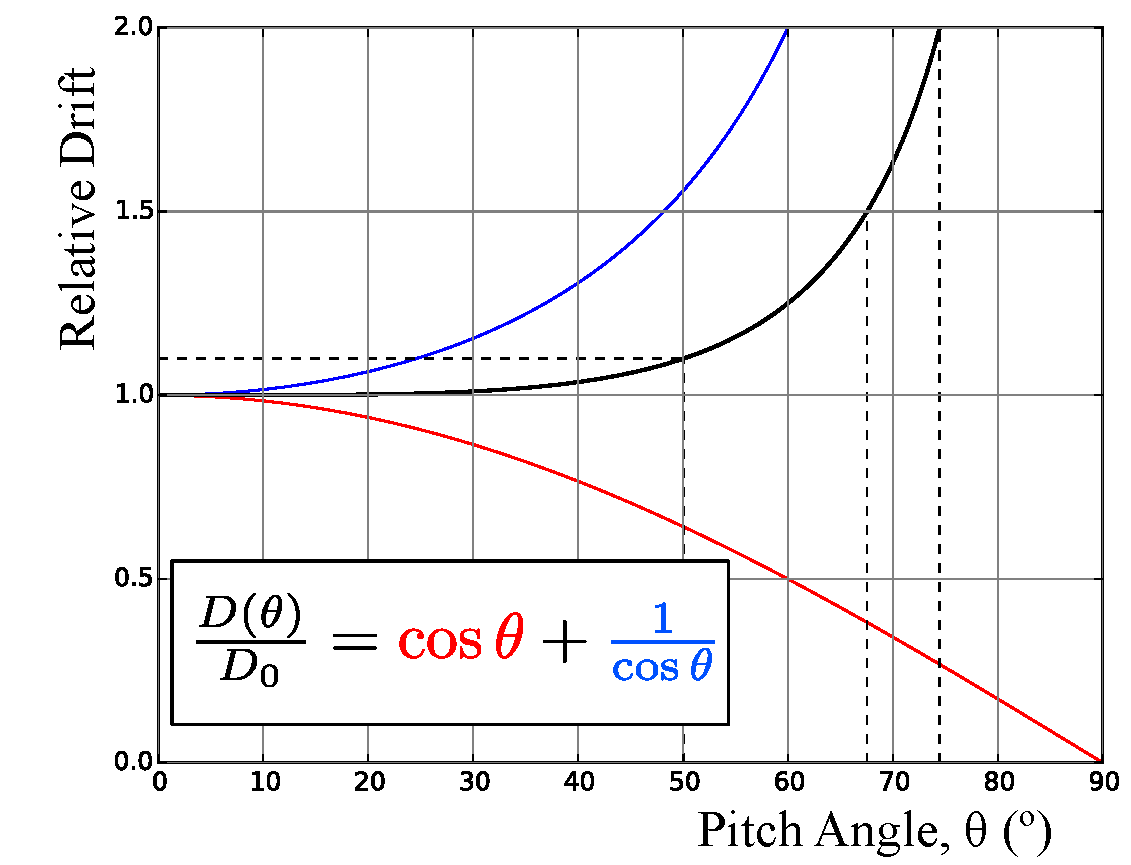
\includegraphics[width=0.6\textwidth]{figs/detector/BentSolenoids_RelativeDrift}
\caption{
Angular dependence of the magnitude of vertical drift in a bent solenoid field.
The total variation (black) remains below 10\% for pitch angles below 50\degree.
}
\figlabel{detector:bent-solenoids:angularDependence}
\end{figure}
}

\newcommand{\FigPhaseII}{
\begin{figure}[t]
\centering
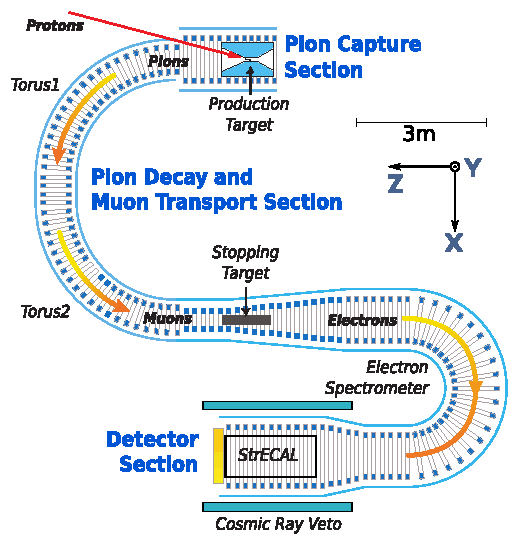
\includegraphics[width=0.9\textwidth]{figs/detector/PhaseII_schematic}
\caption{
Schematic layout of COMET \phaseII. 
The 8 GeV proton beam enters from the top-left, producing (amongst other things) pions.
Pions and muons travelling backwards with respect to the proton beam are then transported around 180 degrees of bent solenoid, during which time most of the pions decay producing an intense muon beam.
About 40\% of these muons then stop in the stopping target (centre of image).
Any electrons coming from  \mueconv are then transported through another 180 degrees of bent solenoid into the detector system.
}
\figlabel{detector:PhaseII:setup}
\end{figure}
}

\newcommand{\FigPhaseI}{
\begin{figure}[t]
\centering
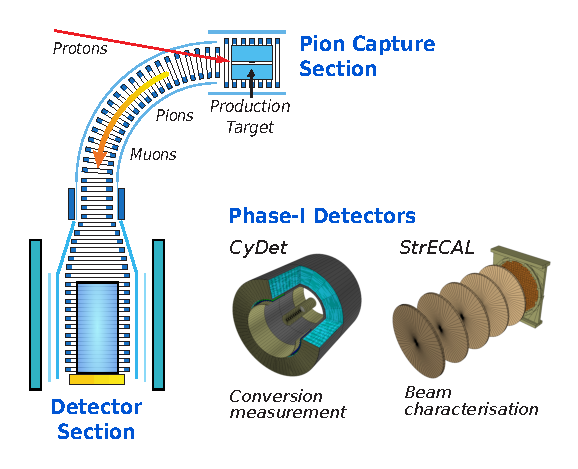
\includegraphics[height=0.4\textheight]{figs/detector/PhaseI_schematic}
\caption{
Schematic layout of COMET \phaseI. 
}
\figlabel{detector:PhaseI:setup}
\end{figure}
}

\newcommand{\TabBackgroundSummary}{
\begin{table}
\begin{tabular}{lldd}
     \hline
     \hline\\[-1.8ex]
     Type           & Background & \multicolumn{2}{c}{Predicted number of events during run} \\
                    &  & \multicolumn{1}{c}{\phaseI \cite{TDR2014}} & \multicolumn{1}{c}{\phaseII \cite{CDRphase2} } \\
     \hline\\[-1.8ex]
     Intrinsic & Muon Decay-in-Orbit                       & 0.01              & 0.15    \\
               & Radiative Muon Capture                    & 0.00056           & <0.001  \\
               & $\mu^-$ Capture w/ n Emission             & <0.001            & <0.001  \\
               & $\mu^-$ Capture w/ Charged Part. Emission & <0.001            & <0.001  \\
     Prompt    & Radiative Pion Capture                    & 0.00023           & 0.05    \\
               & Beam Electrons                            & 0.00083           & <0.1^*  \\
               & Muon Decay in Flight                      & \le0.0002         & <0.0002 \\
               & Pion Decay in Flight                      & \le0.00023        & <0.0001 \\
               & Neutron Induced                           & -                 & 0.024   \\
               & Other beam induced B.G.                   & <2.8\times10^{-6} & -       \\
     Delayed   & Delayed Radiative Pion Capture            & \sim0             & 0.002   \\
               & Anti-proton Induced                        & 0.007             & 0.007   \\
               & Other delayed B.G.                        & \sim0             & -       \\
     Cosmic    & Cosmic Ray Muons                          & -                 & 0.002   \\
               & Electrons from Cosmic Ray Muons           & <0.0001           & 0.002   \\
     \hline\\[-1.8ex]
     \multicolumn{2}{c}{Total background}                      & 0.019         & 0.34    \\
     \multicolumn{2}{c}{Signal (Assuming $B=1\times10^{-16}$)} & 0.31          & 3.8     \\
     \hline
     \hline
\end{tabular}
\caption{
	\CHECK{UPDATE \phaseI values with TDR 2016}
	Backgrounds for COMET \phaseI \cite{TDR2014} and \phaseII \cite{CDRphase2}.
	Prompt backgrounds arise by protons that occur in between bunches and are therefore suppressed by the extinction factor.
	For \phaseI, the recently measured value of $10^{-12}$ was used for the extinction factor, but for \phaseII the older expectation of $10^{-9}$ was used.
}
\tablabel{detector:backgrounds}
\end{table}
}

\newcommand{\FigMuonNuclearParams}{
\begin{figure}[bp]
\centering
\subfloat[][\figlabel{detector:mu-nucl-params:lifetimes}Lifetimes]{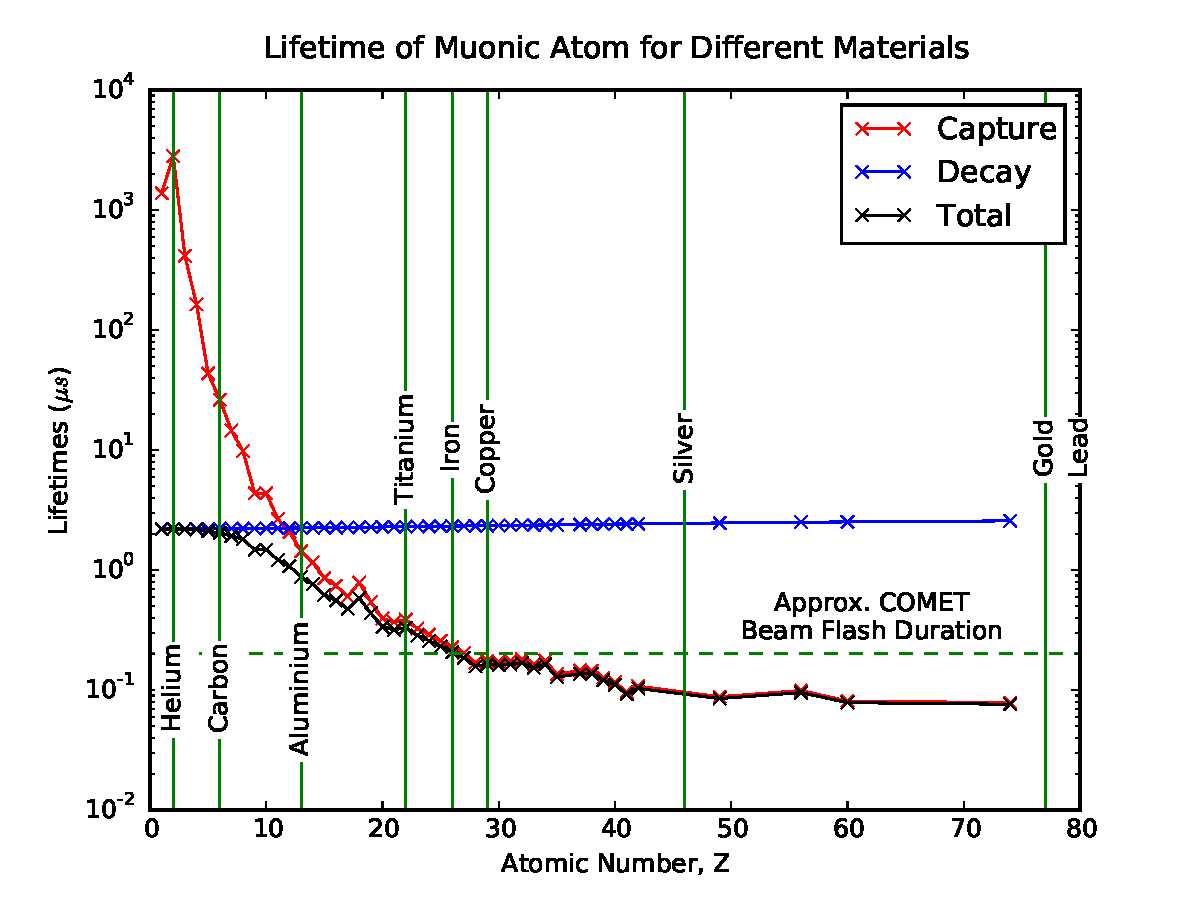
\includegraphics[width=0.9\textwidth]{figs/detector/MuNuclearParams_All_lifetimes.pdf}}\\
\subfloat[][\figlabel{detector:mu-nucl-params:end-point}End-point Shift]{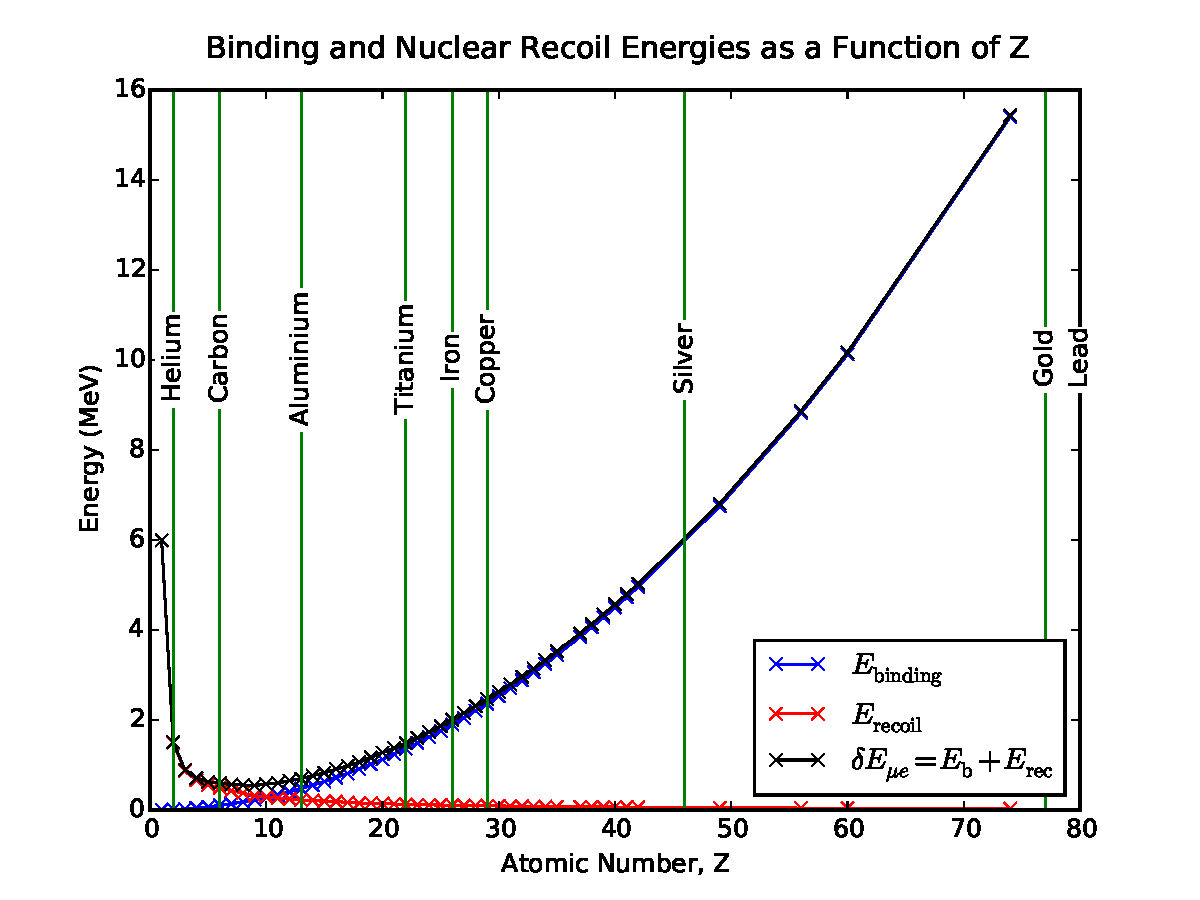
\includegraphics[width=0.49\textwidth]{figs/detector/MuNuclearParams_energies.pdf}}%\hspace{0.5cm}%
\subfloat[][\figlabel{detector:mu-nucl-params:branching-ratio}Branching Fraction]{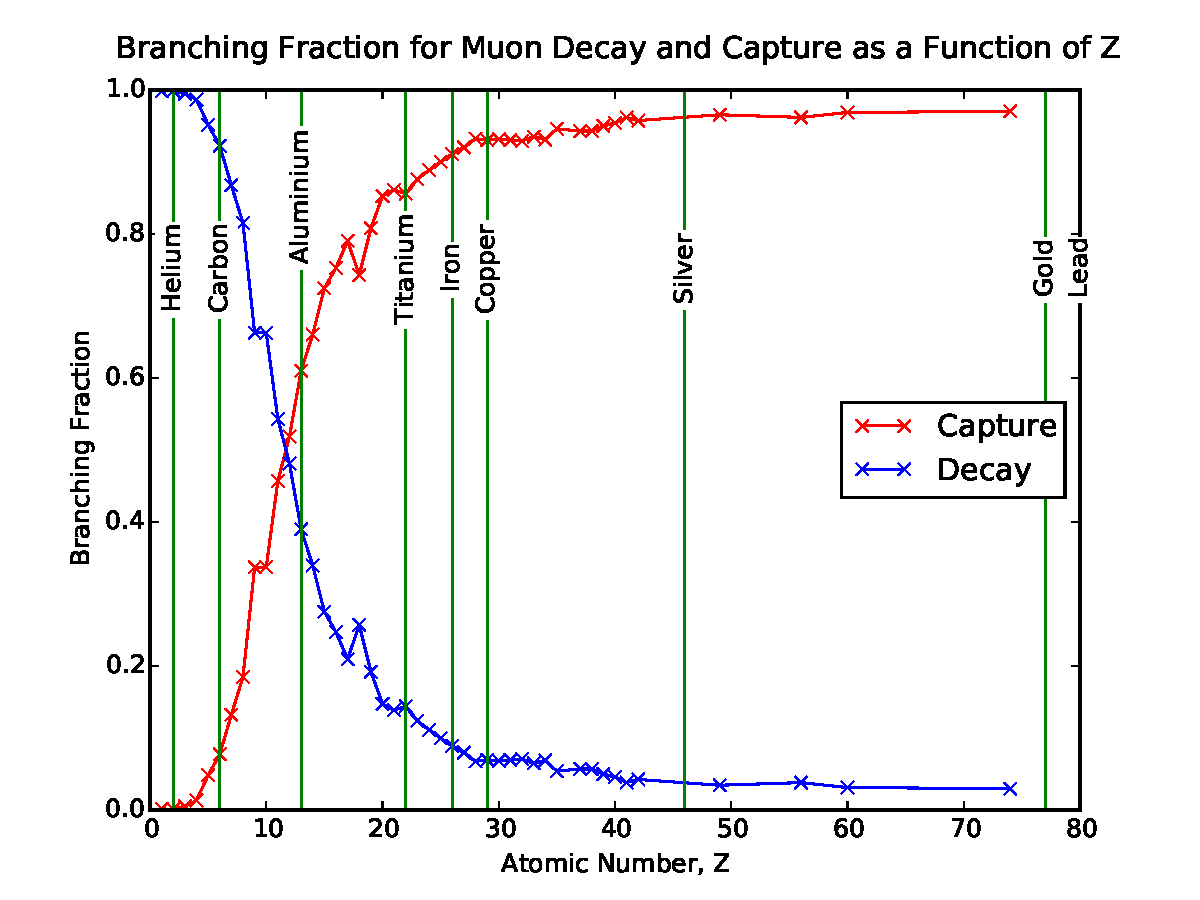
\includegraphics[width=0.49\textwidth]{figs/detector/MuNuclearParams_branching_fraction.pdf}}
\caption{\figlabel{detector:mu-nucl-params}
The effect of changing the atomic number on the branching ratio, lifetime and electron energy spectrum end-point.
For the branching ratio and lifetime plots, the partial rate for muon nuclear capture and decay-in-orbit are shown separately.
The capture and decay rates are taken from the Geant4 \cite{Geant42003} parametrisation for stopped negative muons.  
Only elements for which at least 1 isotope uses a measured value are plotted.
The values for the end-point energy level are calculated using the Bohr model for the muon ground-state binding energy.
}
\end{figure}
}

\chapter{The COMET Experiment}
%\section{Muon to Electron Conversion: Signal and Backgrounds}
% - COMET stands for COherent Muon to Electron Transitions
% - Cite the experimenter's guide by Bob Bernstein

%Introduction:
The aim of the COMET experiment is to search for COherent Muon to Electron Transitions with a single-event-sensitivity of around \sensePII.
This amounts to an improvement of four orders of magnitude compared to the current limit \cite{sindrum2006} which requires some significant changes to the way the experiment operates.

The general experimental goals of COMET are to:
\begin{itemize}
\item stop many muons in aluminium,
\item have a high signal acceptance,
\item suppress potential background sources to well below a single event.
\end{itemize}

At the level of sensitivity desired for COMET these requirements translate to the need for:
\begin{itemize}
\item a very high intensity muon beam,
\item a thin stopping target and low material budget detector,
\item a low energy muon beam,
\item a pulse beam and relatively low-Z stopping target.
\end{itemize}

Realising these goals requires many new experimental techniques and as such COMET has decided to operate in two stages, \phaseI and \phaseII.
\phaseII will realise the final objective of \sensePII, whilst \phaseI is only aiming for \sensePI. 
Although \phaseI will run sooner, since it is heavily motivated by \phaseII, I shall describe \phaseII in more depth first and return \phaseI subsequently.
Firstly however I will discuss some of the key aspects common to both \phaseI and \phaseII.

\section{Proton Beam Energy and Production Target}
\CHECK{Figure for pion vs. antiproton production cross-section}

\section{Particle Transport through Bent Solenoids}
The dynamics of a charged particle in a magnetic field is determined by the Lorentz equation:
\begin{equation}
\vec{F}=\frac{q}{m}\vec{p}\times\vec{B}
\end{equation}
where $q$, $\vec{p}$ and $m$ are the particle's charge, momentum and mass respectively, and $\vec{B}$ is the magnetic field.
In a uniform magnetic field where all field lines are parallel, clearly the motion of the particle follows a helix whose axis is parallel to the field and
with a helical pitch-angle given by:
\begin{equation}
\theta=\tan^{-1}\Big(\frac{P_\mathrm{T}}{P_\mathrm{L}}\Big)
\end{equation}
where $P_\mathrm{T}$ and $P_\mathrm{L}$ are respectively the transverse and longitudinal components of the momentum with respect to the magnetic field.
Such a field can be realised to a high precision by a cylindrical solenoid coil.

If instead one were to bend a solenoid coil, so that it's axis describes a circular arc, two effects are introduced:  firstly, the uniformity of the field is changed
such that a higher magnetic field is found on the inside of the bend, and secondly the field lines also bend.
Each of these changes causes the motion of the particle to deviate from that of a straight solenoid.
Whilst one can think of the particle as following a helix around the field lines still, the centre of this helix can be shown to drift out of the plane of the bending.
Firstly, the radial gradient introduced to the field causes a drift which is proportional to the transverse momentum of the particle.
Secondly, the centrifugal pseudo-force as the particle tracks the now cylindrical field lines, creates a force that acts perpendicularly to the magnetic field.
Since the field lines follow the solenoidal axis, this also produces a vertical drift, proportional to the longitudinal momentum, however.

Taken together, the result is a vertical drift with a velocity given by:
\begin{equation}
\end{equation}

\section{Stopping Target Material and Beam Pulsing}

\section{\COMET \phaseII}
COMET \phaseII will be the final stage of the experiment.
It will make use of all the above techniques

\FigPhaseII
% - Proton beam energy
% - Proton beam timing
% - Production target and capture system
% - Bent Transport system
% - Stopping target
% - Detector system

\section{\COMET \phaseI}
\FigPhaseI
% - Measurement goals
% - StrECAL detector
% - CyDet detector

\section{Status and Schedule}
